\section{Problem Formulation}
In this section we present the general concept of our learning approach. The basic idea is to interpret the folded state of a box as a series of rotation angles along each edge, where the problem of predicting folded state is turned into a problem of predicting these angles. 
\subsection{Definitions and Notations}
As an input to our method, we expect a 2D designed layout of a box represented as a flat triangular mesh $L$. As an output of our method, we deform the input triangular mesh into its 3D realization $R$, according to predicted angles along each of its edges.(An example is shown in Figure~\ref{fig:approximation})\\
\begin{figure}
	\centering
	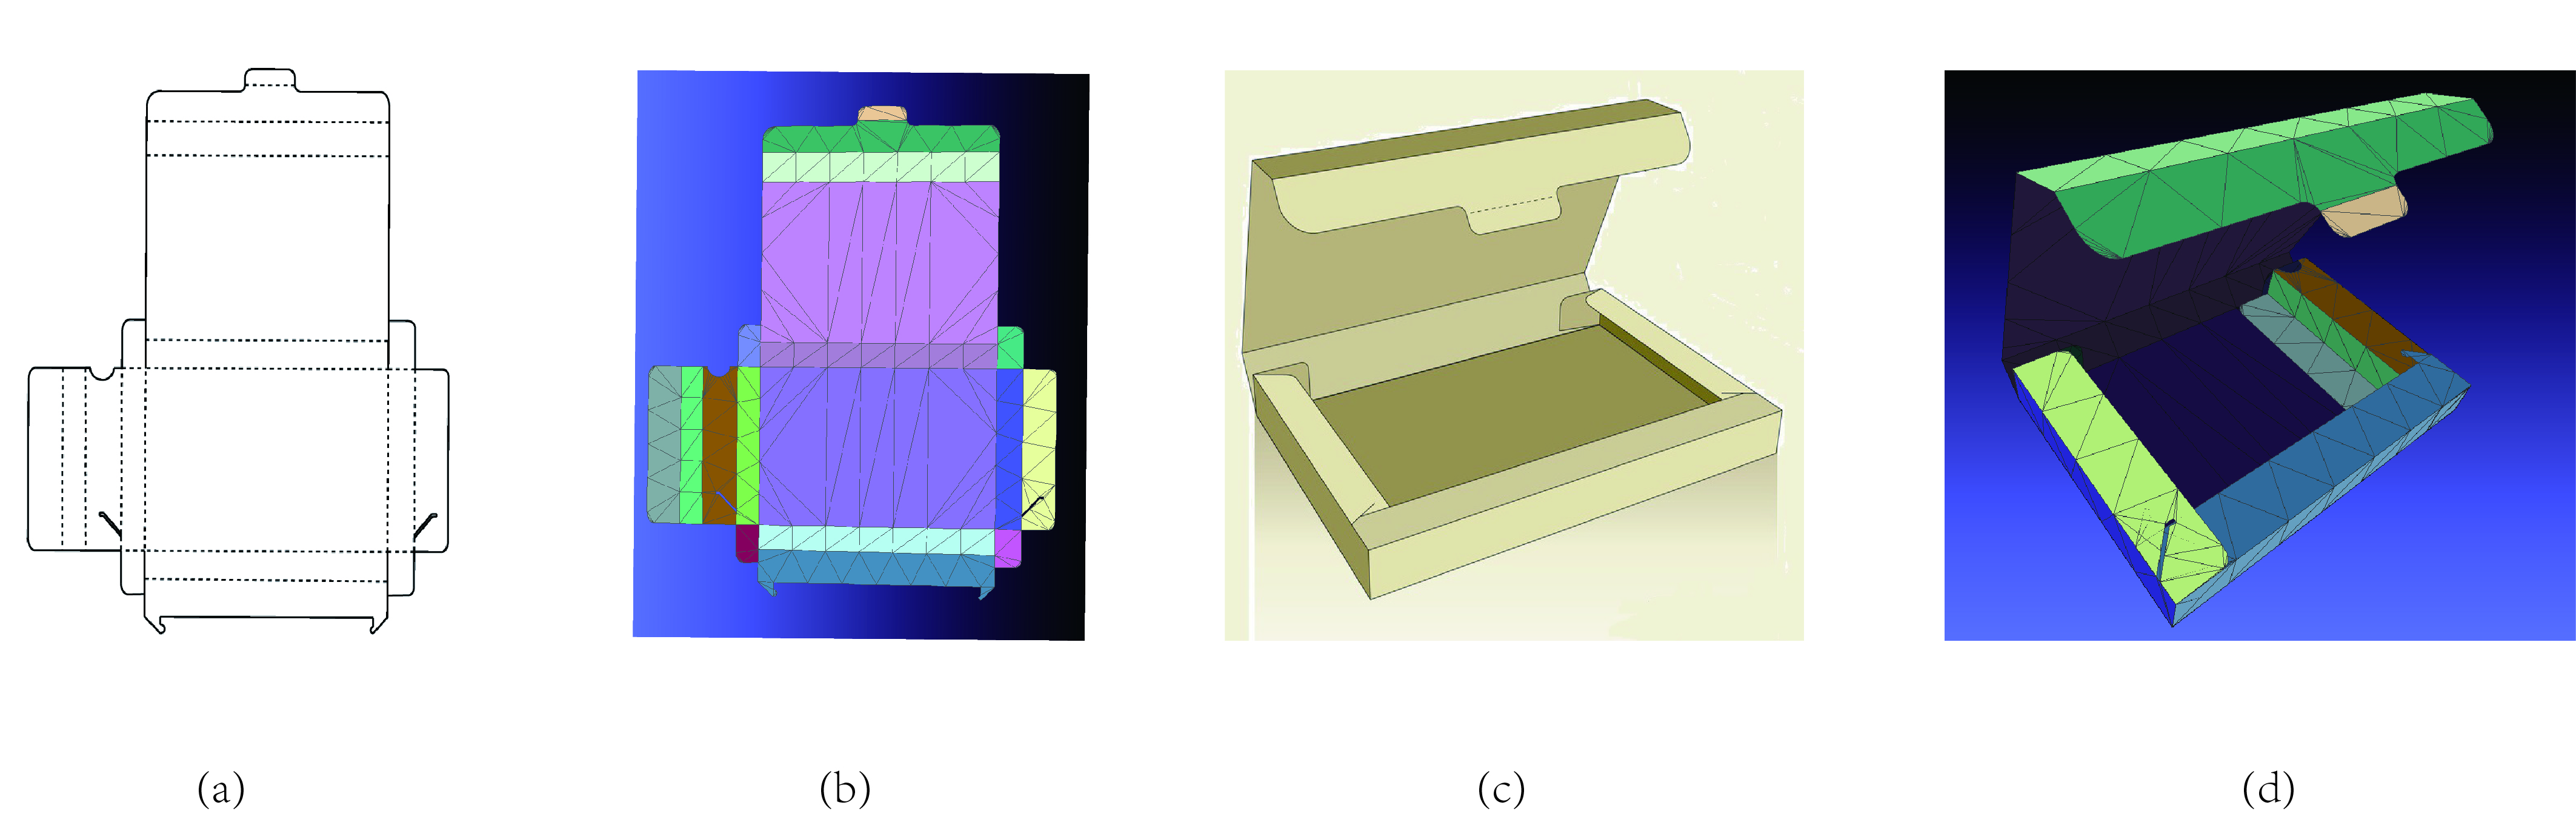
\includegraphics[width=3.0in]{images/approximation.jpg}
	\caption{Given a design layout (a) and its 3D realization (c), we can approximately represent them by triangular mesh as (b) and (d).}
	\label{fig:approximation}
\end{figure}
Without loss of generality, learning to predict the folded state of a box is learning an operator $\mathcal{F}$ that maps every 2D layout to its 3D realization:
\begin{equation}
\mathcal{F}:\{L\}\rightarrow\{R\}
\label{equ:F_0}
\end{equation}
in which $\{L\}$ is the set of all designed layout of boxes represented by 2D triangular meshes and $\{R\}$ is the set of 3D realization of the same boxes represented by deformed triangular meshes. A triangular mesh consists of a set of vertices, edges and faces~$M=(V,E,F)$. The number of vertices, edges and faces varys from one mesh to another. However, a pair of $(L,R)$ as the 2D layout and its correspondent 3D realization share the same topology and therefore has same number of vertices, edges and faces. A flat mesh as a 2D layout from $\{L\}$ has its $z$ component of each vertices set to constant zero: $X_z(v) \equiv 0$ and its normal of each face to $(0,0,1)^T$: $N(e) \equiv (0,0,1)^T$.
\subsection{From Shape Mapping to Functional Mapping}
It is difficult to design a model and a learning scheme to learn the operator in (\ref{equ:F_0}). As we stressed before, the folded state of a box can be represented by a series of rotation angles along each edge which is why we can learn operator $\mathcal{\bar{F}}$ in (\ref{equ:F_1}) instead of $\mathcal{F}$ in (\ref{equ:F_0}):
\begin{equation}
\mathcal{\bar{F}}:\{(X_0,X_1,...,X_n)\}\rightarrow\{\Theta\}
\label{equ:F_1}
\end{equation}
in which the $\{(X_0,X_1,...,X_n)\}$ is a set of feature tensors that is extracted from $\{L\}$ to represent each 2D layout. A feature tensor is composed of n feature functions and a feature function has the form of $X_n:E\rightarrow\mathbb{R}$ which is a real value function that maps each edge of a mesh to a real value. The $\{\Theta\}$ is a set of dihedral angle functions that maps each edge of a mesh to its angle of folded state. One dihedral angle functional has the form of $\Theta:E\rightarrow [0,2\pi]$. To avoid ambiguity, we define the dihedral angle to be the one that the face normal pointed to.({\color{red} {need more elaberation with the definition of ``positive dihedral angle"}})\\
Unfortunately, it is still difficult to learn the operator $\mathcal{\bar{F}}$, since the dimension number of tensors and functions in $\{(X_0,X_1,...,X_n)\}$ and $\{\Theta\}$ varies from one pair of $(L,R)$ to another.\\
To cope with this problem, we approximate each functions as a linear combination of $K$ basis functions $\Phi = \{\phi_k\}$ as $X_n \approx \sum \alpha_k \phi_k$  and $\Theta \approx \sum \theta_k \phi_k$. Each pair of $(L,R)$ shares the same $\Phi$, which allows us to further change the problem into learning $\mathcal{\hat{F}}$ as a mapping from the feature coefficient tensors to dihedral angle coefficients:
\begin{equation}
\mathcal{\hat{F}}:\{(\alpha_k\}_0,\{\alpha_k\}_1,...,\{\alpha_k\}_n)\}\rightarrow\{\{\theta_k\}\}
\label{equ:F_2}
\end{equation}
\subsection{Choice of Basis Functionals}
We construct the basis functionals $\{\Phi\}$ as follows:\\
\subsubsection{Method 1}
Firstly, we construct the edge Laplacian matrix $A$ for a mesh:
\begin{equation}
\left\{
\begin{gathered}
a_{i,j} = w_{i,j} = \exp\{-\frac{d(e_i,e_j)}{\overline{d(e_i,e_j)}}\} \quad \hfill if~(e_i,e_j)~shares~a~vertex. \\
a_{i,i} = -\sum w_{i,j} \quad \hfill \\
a_{i,j} = 0 \quad \hfill otherwise \\
\end{gathered}
\right.
\end{equation}
in which the $d(e_i,e_j)$ is the euclidean distance between the centroid of the edge $e_i$ and edge $e_j$ and $\overline{d(e_i,e_j)}$ is the mean of $d(e_i,e_j)$ on this mesh.\\

\subsubsection{Method 2}
We can also construct the edge Laplacian matrix $A^{'}$ as 
\begin{equation}
\left\{
\begin{gathered}
a_{i,j} = w_{i,j} = \exp\{-\frac{d(e_i,e_j)}{\overline{d(e_i,e_j)}}\} \quad \hfill \\ \quad  \hfill if~(e_i,e_j)~are~in~the~same~face. \\
a_{i,i} = -\sum w_{i,j} \quad \hfill \\
a_{i,j} = 0 \quad \hfill otherwise \\
\end{gathered}
\right.
\end{equation}

where we can remove the effect from little related edges.

\subsubsection{Method 3}
Besides, we have another way to construct the edge Laplacian matrix $A^{''}$ focus on the fold edges $\{e_{f_i}\}$ as

\begin{equation}
\left\{
\begin{gathered}
a_{{f_i},{f_j}} = w_{{f_i},{f_j}} = \exp\{-\frac{d(e_{f_i},e_{f_j})}{\overline{d(e_{f_i},e_j)}}\} \quad \hfill \\ \quad  \hfill if~(e_{f_i},e_{f_j})~satisfy~condition~1. \\
a_{{f_i},-1} = a_{-1,{f_i}} =  w_{{f_i},j} = \exp\{-\frac{d(e_{f_i},e_j)}{\overline{d(e_{f_i},e_{j})}}\} \quad \hfill \\ \quad  \hfill if~(e_{f_i},e_j)~satisfy~condition~2.\\
a_{{f_i},f_i} = -\sum w_{{f_i},{f_j}} \quad \hfill \\
a_{{f_i},{f_j}} = 0 \quad \hfill otherwise \\
\end{gathered}
\right.
\end{equation}


$\overline{d(e_{f_i},e_j)}$ is the average distance of all record distances.  

\textbf{Condition 1:} if $e_{f_i}$ and  $e_{f_j}$ are in the same face, and all of them are the fold edge.

\textbf{Condition 2:} if $e_{f_i}$ and  $e_{j}$ are in the same face, one of them $e_{f_i}$ is the fold edge, and $e_j$ is some cut edge in the same face with $e_{f_i}$.

This method is a wrong implement but we get the best result ever, why?

\subsubsection{Method 3-1}
The dimension of Laplacian is the sum of fold edges' size and cut edges' size which are in the same face with fold edges. 

\subsubsection{Method 3-2}
The dimension of Laplacian is $fn + 1$, $fn$ is the size of fold edges. This method is mean to keep the origin relations between fold edges, and we use the added one row and column to save some covered distance. Figure \ref{fig:method} shows an example of initial distance saved in Laplacian matrix.

\begin{figure}[ht]
	\centering
	\includegraphics[width=3.0in]{images/method3.png}
	\caption{An example shows the initial distance between edge pair of Laplacian matrix by method 3 and 3-2. }
	\label{fig:method}
\end{figure}

\subsubsection{Method 3-3}
Compared with method 3-2, we only set the distance between all fold edges as $\infty$ to observe the influence of last column and row on the corresponding 3D realization.

\subsubsection{Method 3-4}
We construct the similar Laplacian as Method 3-3, to see the influence of last column and row with $size = n$, $n$ is the size of all edges.

Secondly, we calculate $K$ eigenfunctions of $A$ corresponding to the smallest magnitudes of $K$ eigenvalues as $\Phi$ for this mesh.({\color{blue}{We now use ``scipy.sparse.linalg.eigs" in python to solve this problem. It seems that it is also use ``ARPACK" routines as backend the same as other solvers. We choose ``SM" mode to make the solver to choose eigenvalues with smallest magnitudes}})
\subsection{Choice of Features}
We try not to design handcraft features to avoid the loss of information during feature extraction. Therefore, we use the coordinates of vertices from flat meshes as feature functions. For each edge, there is two vertices at each end and two dimension for each vertices in flat meshes, which defines the feature tensor as $(X_{v_0},Y_{v_0},X_{v_1},Y_{v_1})$ for a input mesh.